\chapter{Retrosynthese en strategie in meerdere stappen}\label{ch:b2:retrosynthesis}

Er staat een molecuul op het bord, en nog niemand weet hoe het te maken. Reacties vooruit uitproberen, vanuit
wat er op de plank staat, leidt nergens toe: het zijn er te veel. De chemicus werkt de andere kant op, van het
\omterm{def:b2:retrosynthesis:analysis}{doelmolecuul} terug naar de plank, en knipt op papier één binding tegelijk door, waarbij elke snede een reactie ongedaan maakt die
bekend is om te werken, tot de stukken verbindingen zijn die je kunt kopen. Dit hoofdstuk zet de reacties van
de vorige hoofdstukken om in die achterwaartse redenering, en vraagt dan hoe de route die ze oplevert te beoordelen.

\begin{recall}
\Cref{ch:b2:alkene-redox} tot \cref{ch:b2:wittig}: de reacties die ongedaan gemaakt moeten worden. Het deel van jaar~1:
beschermende groepen en acetalen, grignardreagentia en polariteitsinversie, de williamsonsynthese,
chemoselectiviteit, de oxidatie van alcoholen. Het schoolboek: atoomeconomie.
\end{recall}

\section{Achterwaarts denken}

\begin{definition}[Retrosynthetische analyse]\label{def:b2:retrosynthesis:analysis}
Het molecuul dat gemaakt moet worden, is het \emph{doelmolecuul}\index{doelmolecuul}. \emph{Retrosynthetische analyse}
\index{retrosynthetische analyse} werkt vanuit het doelmolecuul terug naar beschikbare uitgangsstoffen,
in stappen die elk het omgekeerde zijn van een bekende reactie; een retrosynthetische stap wordt geschreven met de
dubbele pijl $\Rightarrow$, gelezen als ``wordt gemaakt uit''.
\end{definition}

\begin{definition}[Disconnectie en synthons]\label{def:b2:retrosynthesis:disconnection}
Een \emph{disconnectie}\index{disconnectie} is het denkbeeldig doorknippen van een binding van het \omterm{def:b2:retrosynthesis:analysis}{doelmolecuul}, het
omgekeerde van een reactie die een binding vormt. Een binding heterolytisch doorknippen geeft twee \emph{synthons}\index{synthon},
geïdealiseerde geladen fragmenten, het ene een donor (nucleofiel, vaak negatief), het andere een acceptor
(elektrofiel, vaak positief). Een \emph{synthetisch equivalent}\index{synthetisch equivalent} is een echt
reagens dat zich als een synthon gedraagt: een grignardreagens voor het carbanion \ce{R-}, een aldehyde voor het
kation $\mathrm{R\overset{+}{C}H{-}OH}$.
\end{definition}

\begin{definition}[Functionele-groepsinterconversie]\label{def:b2:retrosynthesis:fgi}
Een \emph{functionele-groepsinterconversie}\index{functionele-groepsinterconversie} (FGI) is een
retrosynthetische stap die een functionele groep verandert zonder het koolstofskelet te veranderen: een alcohol
uit een keton (door reductie), een alkaanketen uit een alkeen (door hydrogenering), een amine uit een amide.
\end{definition}

\begin{omfigure}
\begin{tikzpicture}[every node/.style={align=center}]
\node (T) at (0,0) {\setchemfig{atom sep=1.7em}\chemfig{Ph-CH(-[2]OH)-CH(-[6]CH_3)-CH_3}};
\node (A) at (-4.6,-2.6) {\ce{PhCHO}\\[1pt] + \ce{(CH3)2CHMgBr}};
\node (B) at (0,-2.6) {\ce{PhMgBr}\\[1pt] + \ce{(CH3)2CHCHO}};
\node (C) at (4.6,-2.6) {\setchemfig{atom sep=1.7em}\chemfig{Ph-C(=[2]O)-CH(-[6]CH_3)-CH_3}};
\node (D) at (4.6,-5.0) {\ce{C6H6}\\[1pt] + \ce{(CH3)2CHCOCl}};
\draw[omretro] (T.south west) -- node[above left, font=\small] {a} (A.north);
\draw[omretro] (T.south) -- node[right, font=\small] {b} (B.north);
\draw[omretro] (T.south east) -- node[above right, font=\small] {FGI} (C.north);
\draw[omretro] (C.south) -- node[right, font=\small] {c} (D.north);
\end{tikzpicture}
\par\vspace{6pt}

{\small Een retrosynthetische boom voor 2-methyl-1-fenylpropaan-1-ol. (a) en (b): de twee \omterm{def:b2:retrosynthesis:disconnection}{disconnecties} van
de binding \ce{C-C} naast het alcoholkoolstofatoom, elk een aldehyde en een grignardreagens. FGI: de alcohol
uit een keton, door reductie; (c) het keton door \omterm{def:b2:aromatic-substitution:friedel-crafts}{friedel-craftsacylering} van benzeen. Elke pijl
leest als ``wordt gemaakt uit''.}
\end{omfigure}

De boom toont de gewoonten van de methode. Een \omterm{def:b2:retrosynthesis:disconnection}{disconnectie} wordt gekozen bij een binding naast een functionele
groep, omdat reacties daar bindingen maken. Elke snede wordt gecontroleerd door de \omterm{def:b2:retrosynthesis:disconnection}{synthons} op te schrijven en
er echte reagentia voor te vinden. En er is zelden één antwoord: de boom vertakt zich, en de takken worden
op het einde beoordeeld (\cref{sec:b2:retrosynthesis:judging}).

\begin{omfigure}
\begin{center}
\small
\renewcommand{\arraystretch}{1.25}
\begin{tabular}{lll}
\hline
\omterm{def:b2:retrosynthesis:disconnection}{Synthon} & Soort & \omterm{def:b2:retrosynthesis:disconnection}{Synthetisch equivalent} \\
\hline
\ce{R-} (alkyl, aryl) & donor & \ce{RMgBr}, \ce{RLi}, \ce{R2CuLi} (geconjugeerd) \\
$\mathrm{^-CH_2COR}$ & donor & het \omterm{def:b2:enolates-aldol:enolate}{enolaat} van \ce{CH3COR}, of ethyl-3-oxobutanoaat \\
$\mathrm{^-C{\equiv}N}$ & donor & \ce{NaCN} \\
$\mathrm{R\overset{+}{C}H{-}OH}$ & acceptor & het aldehyde \ce{RCHO} \\
$\mathrm{R\overset{+}{C}{=}O}$ & acceptor & het \omterm{def:b2:acyl-substitution:derivative}{acylchloride} \ce{RCOCl}, een ester \\
\ce{R+} (primair) & acceptor & het halogenide \ce{RBr} (bimoleculaire substitutie) \\
$\mathrm{^+CH_2CH_2COR}$ & acceptor & het enon \ce{CH2=CHCOR} (\omterm{def:b2:conjugate-additions:addition-modes}{geconjugeerde additie}) \\
\hline
\end{tabular}
\end{center}

{\small Gangbare \omterm{def:b2:retrosynthesis:disconnection}{synthons} en hun synthetische equivalenten. De donorsynthons zijn carbanionen, de
acceptorsynthons carbokationen; de echte reagentia dragen dezelfde polariteit zonder de volledige lading.}
\end{omfigure}

\section{Disconnecties met één groep}

Een \omterm{def:b2:retrosynthesis:disconnection}{disconnectie} met één groep knipt een binding naast één enkele functionele groep door. Bij een binding \ce{C-O} of \ce{C-N}
van een ether, ester of amine gaat de snede tussen koolstof en het heteroatoom: het heteroatoom is
de donor, het koolstofatoom de acceptor (een williamsonsynthese, een \omterm{def:b2:acyl-substitution:esterification}{verestering}, een amidevorming).
Bij een binding \ce{C-C} legt de functionele groep de polariteit van de \omterm{def:b2:retrosynthesis:disconnection}{synthons} vast: naast een
alcoholkoolstofatoom is het alcoholkoolstofatoom de acceptor (een aldehyde of keton) en het andere koolstofatoom de donor (een
organometaalverbinding); naast een carbonylgroep is het $\alpha$-koolstofatoom de donor (een \omterm{def:b2:enolates-aldol:enolate}{enolaat}).

De meeste van deze reacties vragen het juiste oxidatieniveau op de juiste plaats, dus FGI's tussen
oxidatieniveaus zijn de gewoonste stappen van een route: alkeen, alcohol, aldehyde of keton, zuur. Eén ervan bleef
open in het deel van jaar~1: de oxidatie van een primaire alcohol bij het aldehyde laten stoppen.

\begin{proposition}[Milde oxidaties]\label{prop:b2:retrosynthesis:mild-oxidation}
Een primaire alcohol wordt geoxideerd tot het aldehyde, zonder door te gaan tot het zuur, door een oxidator die gebruikt wordt in een
watervrij organisch oplosmiddel: pyridiniumchloorchromaat in dichloormethaan, de swernoxidatie
(dimethylsulfoxide geactiveerd door oxalylchloride, daarna triethylamine, bij lage temperatuur) of het
Dess--Martin-perjodinaan. In water oxideren chroom(VI) of permanganaat haar tot het carbonzuur.
\end{proposition}

\begin{proof}[Redenering]
Deze oxidatoren halen het waterstofatoom weg van de binding \ce{C-H} op het koolstofatoom dat een \ce{OH} draagt. Het gevormde
aldehyde heeft zo'n groep niet. In water staat een aldehyde echter in evenwicht met zijn hydraat
\ce{RCH(OH)2}, dat opnieuw een \ce{OH} heeft op een koolstofatoom met een waterstofatoom: het hydraat wordt geoxideerd
zoals een alcohol, tot het zuur. Zonder water vormt zich geen hydraat, en de oxidatie stopt bij het
aldehyde.
\end{proof}

\section{Disconnecties met twee groepen}

Wanneer het \omterm{def:b2:retrosynthesis:analysis}{doelmolecuul} twee functionele groepen heeft, gebruikt de beste \omterm{def:b2:retrosynthesis:disconnection}{disconnectie} meestal beide: de binding wordt zo
doorgeknipt dat de ene groep de donor bepaalt en de andere de acceptor. De afstand tussen de groepen,
in koolstofatomen geteld van het ene gefunctionaliseerde koolstofatoom tot het andere, beide inbegrepen, zegt welke reactie je gebruikt.

\begin{proposition}[Patronen en hun reacties]\label{prop:b2:retrosynthesis:patterns}
De relaties tussen twee groepen komen als volgt overeen met de reacties van de vorige hoofdstukken. De
oneven relaties (1,3 en 1,5) passen bij de natuurlijke polariteiten van de carbonylchemie; de even (1,4
en 1,6) niet, en die vragen polariteitsinversie of het openknippen van een ring.
\end{proposition}


\begin{proof}[Redenering]
In de carbonylchemie is het carbonylkoolstofatoom een acceptor en het $\alpha$-koolstofatoom een donor, en een enon
voegt een acceptor toe op zijn $\beta$-koolstofatoom. Een \omterm{def:b2:enolates-aldol:enolate}{enolaat} (donor op $\alpha$) op een carbonylgroep (acceptor op het
carbonylkoolstofatoom) verbindt de koolstofatomen 1 en 2 van een 1,3-patroon: \omterm{def:b2:enolates-aldol:aldol}{aldol} en Claisen. Een \omterm{def:b2:enolates-aldol:enolate}{enolaat} op het $\beta$-koolstofatoom
van een enon bouwt een 1,5-patroon: Michael, daarna Robinson. Bij een 1,4-patroon laat de snede een
$\alpha$-koolstofatoom als acceptor achter; geen gewoon carbonylreagens biedt die polariteit, maar een
$\alpha$-broomketon wel, omdat bromide op dat koolstofatoom een vertrekkende groep is. Een 1,6-dicarbonylverbinding is een cyclohexeen dat geopend wordt
door \omterm{def:b2:alkene-redox:cleavage}{ozonolyse} (\cref{prop:b2:alkene-redox:ozonolysis}), en het cyclohexeen wordt gemaakt door een
\omterm{def:b2:frontier-orbitals:diels-alder}{diels-alderreactie} (\cref{def:b2:frontier-orbitals:diels-alder}).
\end{proof}

\begin{omfigure}
\begin{center}
\small
\renewcommand{\arraystretch}{1.25}
\begin{tabular}{lll}
\hline
Patroon in het \omterm{def:b2:retrosynthesis:analysis}{doelmolecuul} & \omterm{def:b2:retrosynthesis:disconnection}{Disconnectie} & Reactie \\
\hline
$\beta$-hydroxycarbonyl (1,3) & binding $\alpha$--$\beta$ & \omterm{def:b2:enolates-aldol:aldol}{aldoladditie} \\
$\alpha,\beta$-onverzadigd carbonyl & \ce{C=C} & \omterm{def:b2:enolates-aldol:aldol}{aldolcondensatie} \\
1,3-dicarbonyl & C(O)--C$\alpha$ & \omterm{def:b2:enolates-aldol:claisen}{claisencondensatie} \\
1,5-dicarbonyl & C$\alpha$--C$\beta$ van de acceptor & \omterm{def:b2:conjugate-additions:michael}{michaeladditie} \\
cyclohex-2-een-1-on & ring-\ce{C=C}, dan michaelbinding & \omterm{def:b2:conjugate-additions:robinson}{robinsonannulatie} \\
cyclohexeen & twee ringbindingen \ce{C-C} & \omterm{def:b2:frontier-orbitals:diels-alder}{diels-alderreactie} \\
alkeen op vaste plaats & \ce{C=C} & wittig- of HWE-reactie \\
1,4-dicarbonyl & centrale \ce{C-C} & \omterm{def:b2:enolates-aldol:enolate}{enolaat} + $\alpha$-halogeenketon \\
1,6-dicarbonyl & uiteinden verbinden & \omterm{def:b2:alkene-redox:cleavage}{oxidatieve splitsing} van cyclohexeen \\
\hline
\end{tabular}
\end{center}

{\small De \omterm{def:b2:retrosynthesis:disconnection}{disconnecties} met twee groepen. De eerste zes gebruiken de normale polariteit: een \omterm{def:b2:enolates-aldol:enolate}{enolaat} (donor) op een
carbonylgroep of een enon (acceptor). Het 1,4-patroon vraagt dat een koolstofatoom $\alpha$ ten opzichte van een carbonylgroep de
acceptor is, het omgekeerde van zijn gewone rol, en dat levert een $\alpha$-halogeenketon.}
\end{omfigure}

\begin{method}[Een retrosynthetische analyse]\label{met:b2:retrosynthesis:retrosynthesis}
\begin{enumerate}
  \item Som de functionele groepen van het \omterm{def:b2:retrosynthesis:analysis}{doelmolecuul} op en hun relaties (1,2; 1,3; \dots).
  \item Overweeg FGI's die een patroon met een goede \omterm{def:b2:retrosynthesis:disconnection}{disconnectie} zouden geven (een alcohol uit een keton, een
        alkaanketen uit een alkeen).
  \item Kies strategische bindingen: naast een functionele groep, nabij het midden van het molecuul, op een
        vertakkingspunt of waar een ring aan een keten vastzit, zodat de stukken ongeveer even groot zijn.
  \item Schrijf de \omterm{def:b2:retrosynthesis:disconnection}{synthons} op, en daarna hun synthetische equivalenten; verwerp een snede zonder echt reagens.
  \item Controleer de chemoselectiviteit: welke andere groep zou met elk reagens reageren? Plan een bescherming
        of verander de volgorde van de stappen.
  \item Herhaal dit voor elk stuk tot alle stukken beschikbaar zijn; schrijf daarna de route vooruit op, met reagentia en
        omstandigheden.
\end{enumerate}
\end{method}

\section{Beschermende groepen in een route}

Een route vraagt vaak een reagens dat een tweede groep van het molecuul zou aanvallen. Het deel van jaar~1
beschermde aldehyden en ketonen als acetalen. Een route kiest uit verscheidene beschermende groepen, die elk
onder hun eigen omstandigheden verwijderd worden: acetalen (verwijderd door waterig zuur), silylethers van alcoholen (verwijderd door
fluoride-ionen), benzylethers (verwijderd door hydrogenolyse over palladium), carbamaten van aminen zoals
de \textit{tert}-butoxycarbonylgroep (verwijderd door zuur), en esters (verwijderd door base).

\begin{definition}[Orthogonale bescherming]\label{def:b2:retrosynthesis:orthogonal}
Een set \emph{orthogonale beschermende groepen}\index{orthogonale beschermende groepen} is een set beschermende
groepen die elk verwijderd kunnen worden onder omstandigheden die alle andere intact laten, zodat de functies die ze maskeren
één voor één vrijgemaakt kunnen worden, in elke volgorde.
\end{definition}

\begin{method}[Beschermen in een route]\label{met:b2:retrosynthesis:protect-in-route}
\begin{enumerate}
  \item Som voor elke stap de groepen op die het reagens naast de bedoelde groep zou aanvallen.
  \item Probeer eerst bescherming te vermijden: verander de volgorde van de stappen, of gebruik een selectiever reagens
        (een boorhydride in plaats van een hydride voor een keton naast een ester).
  \item Kies anders een groep die in elke stap stabiel is tot ze verwijderd wordt, en die verwijderd kan worden onder omstandigheden die het
        molecuul verdraagt.
  \item Kies bij verscheidene groepen die afzonderlijk vrijgemaakt moeten worden een orthogonale set.
  \item Zoek een stap die een groep gratis verwijdert: een hydrogenering die toch al gepland is, verwijdert ook een
        benzylether.
  \item Tel: elke bescherming kost twee stappen en hun rendementen.
\end{enumerate}
\end{method}

\section{Een route beoordelen}\label{sec:b2:retrosynthesis:judging}

\begin{proposition}[Totaal rendement]\label{prop:b2:retrosynthesis:overall-yield}
Het totale rendement van een lineaire reeks stappen is het product van de rendementen per stap:
$\rho = \rho_1 \rho_2 \cdots \rho_n$. Bij $n$ stappen met hetzelfde rendement $\rho_1$ geldt $\rho = \rho_1^{\,n}$.
\end{proposition}

\begin{proof}
Stap $k$ zet de hoeveelheid $n_{k-1}$ van zijn uitgangsstof om in $n_k = \rho_k\, n_{k-1}$ product
(rendementen betrokken op hoeveelheden van het intermediair, alle andere reagentia in voldoende hoeveelheid). Door inductie is
$n_n = \rho_n \rho_{n-1} \cdots \rho_1\, n_0$, en het totale rendement $n_n/n_0$ is het product.
\end{proof}

\begin{omfigure}
\begin{tikzpicture}
\begin{axis}[width=0.75\linewidth, height=5.4cm, xmin=0, xmax=20, ymin=0, ymax=100,
  xlabel={aantal stappen $n$}, ylabel={totaal rendement (\%)}, label style={font=\small},
  tick label style={font=\scriptsize}, xtick={0,5,10,15,20}, grid=major, grid style={black!12},
  legend style={font=\scriptsize, at={(0.98,0.98)}, anchor=north east}, legend cell align=left]
\addplot[omDef, thick] table[x=n, y=r95] {figdata/out/bachelor-2-overall-yield.dat};
\addplot[omThm, thick] table[x=n, y=r90] {figdata/out/bachelor-2-overall-yield.dat};
\addplot[omMeth, thick] table[x=n, y=r80] {figdata/out/bachelor-2-overall-yield.dat};
\addplot[black!60, thick, dashed] table[x=n, y=r70] {figdata/out/bachelor-2-overall-yield.dat};
\legend{95~\% per stap, 90~\% per stap, 80~\% per stap, 70~\% per stap}
\end{axis}
\end{tikzpicture}
\par\vspace{4pt}

{\small Totaal rendement van een lineaire route tegen haar aantal stappen, voor vier rendementen per stap
(\cref{prop:b2:retrosynthesis:overall-yield}). Tien stappen van elk 90~\% houden 35~\% van het materiaal over; tien
stappen van 70~\% minder dan 3~\%.}
% figdata: bachelor-2/overall-yield.py
\end{omfigure}

De productregel verklaart waarom korte routes winnen, waarom een bescherming (twee extra stappen) nooit gratis is, en waarom
chemici liever twee helften afzonderlijk bouwen en ze laat verbinden: de lange route loopt dan in twee
kortere takken, en de verliezen van de ene tak vermenigvuldigen die van de andere niet. Naast rendement en
lengte wordt een route beoordeeld op \omterm{def:b2:continuous-reactors:selectivity}{selectiviteit} (elke stap hoort één product te geven), op de kosten en de gevaren
van haar reagentia, op het afval dat ze oplevert (de atoomeconomie van elke stap en de oplosmiddelen van de
zuiveringen), en op hoe gemakkelijk elke stap opgeschaald kan worden.

\begin{history}[Achterwaarts werken, expliciet gemaakt]
\begin{minipage}[t]{0.2\linewidth}
\vspace{0pt}
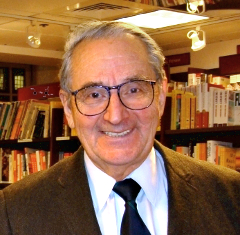
\includegraphics[width=\linewidth]{images/book3/corey.jpg}
\end{minipage}\hfill
\begin{minipage}[t]{0.76\linewidth}
\vspace{0pt}
Chemici hadden altijd al achterwaarts geredeneerd vanuit hun doelmoleculen, maar Elias James Corey maakte vanaf de jaren 1960
van die gewoonte expliciete regels: de \omterm{def:b2:retrosynthesis:disconnection}{disconnectie}, het \omterm{def:b2:retrosynthesis:disconnection}{synthon}, de retrosynthetische pijl, en
zelfs computerprogramma's die ze toepasten. Hij kreeg in 1990 de Nobelprijs voor de Scheikunde voor de theorie
en methodologie van de organische synthese. (Foto: door Trvthchem, CC0, Wikimedia Commons.)
\end{minipage}
\end{history}

\begin{safety}{\ghs[5mm]{GHS02}\,\ghs[5mm]{GHS03}\,\ghs[5mm]{GHS05}\,\ghs[5mm]{GHS06}\,\ghs[5mm]{GHS07}\,\ghs[5mm]{GHS08}}
Oxalylchloride is corrosief, giftig en reageert met water, waarbij waterstofchloride vrijkomt; de
swernoxidatie maakt koolstofmonoxide en onwelriekend dimethylsulfide vrij, en wordt daarom in een zuurkast uitgevoerd.
Het Dess--Martin-perjodinaan is een oxidator en mag niet verhit worden. Chroom(VI)-reagentia worden nu
vermeden waar er een alternatief bestaat.
% ledger: ghs:oxalyl-chloride, ghs:DMSO, ghs:DMP
\end{safety}

\section{Oefeningen}

\begin{exercise}[$\star$]\label{exo:b2:retrosynthesis:1}
Maak van elke alcohol een \omterm{def:b2:retrosynthesis:disconnection}{disconnectie} in een carbonylverbinding en een grignardreagens (geef elke mogelijkheid):
2-fenylpropaan-2-ol, pentaan-3-ol, 1-cyclohexylethanol, 2-methylbutaan-2-ol, 1-fenylethanol.
\end{exercise}

\begin{exercise}[$\star$]\label{exo:b2:retrosynthesis:2}
Geef voor de \omterm{def:b2:retrosynthesis:disconnection}{disconnectie} van 1-fenylethanol aan de binding \ce{C-C} de twee \omterm{def:b2:retrosynthesis:disconnection}{synthons}, zeg welk de
donor is, en geef voor elk een \omterm{def:b2:retrosynthesis:disconnection}{synthetisch equivalent}.
\end{exercise}

\begin{exercise}[$\star$]\label{exo:b2:retrosynthesis:3}
Een route in vijf stappen heeft rendementen per stap van 90, 85, 80, 95 en 70~\%. Bereken haar totale rendement.
\end{exercise}

\begin{exercise}[$\star$]\label{exo:b2:retrosynthesis:4}
Ethyl-4-oxopentanoaat moet omgezet worden in 5-hydroxypentaan-2-on. Plan de route met een beschermende
groep, en zeg waarom die nodig is.
\end{exercise}

\begin{exercise}[$\star\star$]\label{exo:b2:retrosynthesis:5}
Stel een retrosynthese voor van butaan-1,3-diol uit verbindingen met ten hoogste twee koolstofatomen, met een FGI en een
\omterm{def:b2:retrosynthesis:disconnection}{disconnectie} met twee groepen.
\end{exercise}

\begin{exercise}[$\star\star$]\label{exo:b2:retrosynthesis:6}
Maak een \omterm{def:b2:retrosynthesis:disconnection}{disconnectie} van 1-(cyclohex-3-een-1-yl)ethaan-1-on via een \omterm{def:b2:frontier-orbitals:diels-alder}{diels-alderreactie}.
\end{exercise}

\begin{exercise}[$\star\star$]\label{exo:b2:retrosynthesis:7}
Maak een \omterm{def:b2:retrosynthesis:disconnection}{disconnectie} van 4,4-dimethylcyclohex-2-een-1-on via een \omterm{def:b2:conjugate-additions:robinson}{robinsonannulatie}.
\end{exercise}

\begin{exercise}[$\star\star$]\label{exo:b2:retrosynthesis:8}
1-Fenylbutaan-1-on kan in één stap gemaakt worden door een \omterm{def:b2:aromatic-substitution:friedel-crafts}{friedel-craftsacylering}, of in twee uit benzaldehyde.
Schrijf beide routes op en vergelijk ze.
\end{exercise}

\begin{exercise}[$\star\star$]\label{exo:b2:retrosynthesis:9}
Men wil hexanal uit hexaan-1-ol. Welke reagentia geven het, en welk zou in plaats daarvan hexaanzuur
geven? Leg uit.
\end{exercise}

\begin{exercise}[$\star\star\star$]\label{exo:b2:retrosynthesis:10}
In 4-aminobutaan-1-ol moet het amine eerst in één stap met een \omterm{def:b2:acyl-substitution:derivative}{acylchloride} reageren, en de alcohol
later met een ander. Stel een orthogonaal paar beschermende groepen voor en de volgorde van de stappen.
\end{exercise}

\begin{exercise}[$\star\star\star$]\label{exo:b2:retrosynthesis:11}
Stel een synthese voor van hexaan-2,5-dion, een 1,4-dicarbonylverbinding, uit ethyl-3-oxobutanoaat.
\end{exercise}

\begin{exercise}[$\star\star\star$]\label{exo:b2:retrosynthesis:12}
6-Methylhept-5-een-2-on, \ce{(CH3)2C=CHCH2CH2COCH3}, is een tussenproduct voor geurstoffen. Stel een volledig plan voor
uit ethyl-3-oxobutanoaat en een halogenide: retrosynthese, voorwaartse route, en de stap die de
estergroep verwijdert.
\end{exercise}

\section{Probleem: frambozenketon}

\begin{problem}[{Weekendprobleem --- de retrosynthese van een aromastof, het fenol en de vraag of
het beschermd moet worden, een alternatief met palladium, en de beoordeling van de routes}]
\label{pb:b2:retrosynthesis:1}
Frambozenketon, 4-(4-hydroxyfenyl)butaan-2-on, komt voor in frambozen en andere vruchten en wordt gebruikt
als aromastof en in de parfumerie. Gegevens voor de oefening: rendementen per stap van de aldolroute, 85~\% (condensatie)
en 92~\% (hydrogenering). Molaire massa's (\unit{g/mol}): C 12.011, H 1.008, O 15.999, N 14.007,
I 126.90. De $\mathrm pK_a$ van fenol is 9.99.
% ledger: use:raspberry-ketone, aw:C, aw:H, aw:O, aw:N, aw:I, pka:phenol, ghs:raspberry-ketone, ghs:4-iodophenol, ghs:MVK

\medskip
\noindent\textbf{Deel I --- Retrosynthese.}
\begin{enumerate}
  \item Teken het \omterm{def:b2:retrosynthesis:analysis}{doelmolecuul} en geef zijn functionele groepen.
  \item Welke FGI zet de eenheid \ce{ArCH2CH2CO} om in een patroon met een bekende \omterm{def:b2:retrosynthesis:disconnection}{disconnectie}?
  \item Schrijf het verkregen onverzadigde keton op, met zijn geometrie.
  \item Welk patroon met twee groepen bevat het, en welke reactie maakt het?
  \item Geef de twee uitgangsstoffen.
  \item Waarom geeft deze gekruiste \omterm{def:b2:enolates-aldol:aldol}{aldolreactie} één hoofdproduct?
  \item Schrijf de voorwaartse route in twee stappen op, met de omstandigheden.
\end{enumerate}

\medskip
\noindent\textbf{Deel II --- Het fenol.}
\begin{enumerate}[resume]
  \item In welke vorm is 4-hydroxybenzaldehyde aanwezig in waterig natriumhydroxide? Gebruik de
        $\mathrm pK_a$.
  \item Hoe verandert die vorm de elektrofiliciteit van het aldehyde?
  \item Als het fenol beschermd was, welke groep zou de tweede stap dan gratis verwijderen? Leg uit.
  \item Tel de stappen van de route met die bescherming.
  \item Loopt de benzeenring gevaar bij de hydrogenering?
  \item Beschermen of niet? Besluit.
\end{enumerate}

\medskip
\noindent\textbf{Deel III --- Een alternatief met palladium.}
\begin{enumerate}[resume]
  \item Maak een \omterm{def:b2:retrosynthesis:disconnection}{disconnectie} van het onverzadigde keton aan de binding tussen de ring en de keten: welke
        heckpartners?
  \item Schrijf de heckreactie op met triethylamine als base.
  \item Op welk koolstofatoom van but-3-een-2-on komt de arylgroep terecht, en waarom?
  \item Geef de stappen van de \omterm{def:b2:catalytic-cycles:cycle}{katalytische cyclus}.
  \item Bereken de atoomeconomie van de heckstap, triethylamine meegerekend.
  \item Bereken de atoomeconomie van de \omterm{def:b2:enolates-aldol:aldol}{aldolcondensatie}.
\end{enumerate}

\medskip
\noindent\textbf{Deel IV --- De routes beoordelen.}
\begin{enumerate}[resume]
  \item Wat is de atoomeconomie van de hydrogenering?
  \item Bereken de totale atoomeconomie van de aldolroute.
  \item Welke dubbele binding reduceert de hydrogenering, en waarom blijft het keton intact?
  \item Vergelijk de reagentia van de twee routes op kosten en gevaren.
  \item Welke route zou je kiezen?
  \item Wat zou een derde stap van 90~\% met het totale rendement doen?
  \item Geef het totale rendement van de aldolroute in twee stappen.
\end{enumerate}
\end{problem}
